\let\textcircled=\pgftextcircled
\chapter{Introduction}
\label{chap:intro}

\initial{N}atural Language Processing (NLP) is being increasingly used by different organisations to  improve the dialogue with the customers, efficiently analyse the opinion about a number of topics while using the existing social media tools, and offer additional services which would not have been possible without computational linguistics - such as speech recognition. In a way, Natural Language Processing allows the organisations using social media to have an additional sensor of the public opinion without asking people to give explicit feedback.

The huge amount of unstructured data that is being created by both humans and machines daily has been one of the major unsolved problems of Computer Science since the early days of digital computing. Natural Language Processing allows to systematise, organise and process it. One of the applications of these techniques could be to create a seamless experience for the people living in a certain council area to communicate with the estate, provide feedback and receive answers to their questions. The main advantage of such a technique is the fact that such organisations can use popular social media platforms that already exist such as Twitter and Facebook and can avoid setting up their own separate communication channel. 


\section{Falkirk Council and Grangemouth}
\label{sec:falkirk}

Grangemouth is a Scottish town and a part of the Falkirk council area. Its population was estimated to be around 17000 people by the 2011 census \cite{falkirkcensus}. The growth of the town has mostly been defined by its location: Grangemouth was a port and used to play an important part in trading and the transportation of imported goods using the Forth and Clyde Canal. Nowadays, a lot of the town production is defined by the oil refinery, which is commonly called Grangemouth, too, and has changed its owners several times in the last decades. 

\subsection{Environmental Issues in Grangemouth}
\label{subsec:environment}

\begin{figure}
    \centering
    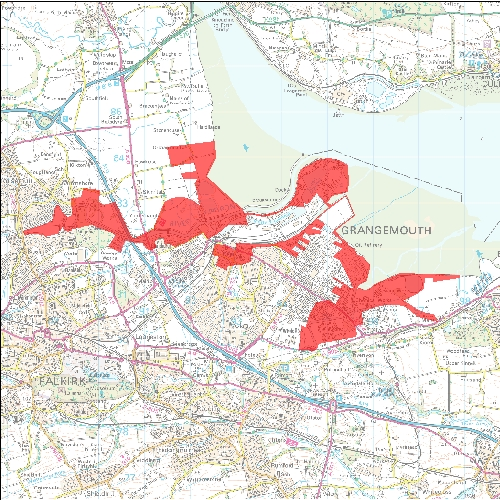
\includegraphics[width=\textwidth]{data/grangemouthflooding}
    \caption{Target area that SEPA will issue a flood warning for (from http://www.sepa.org.uk/)}
    \label{fig:grangemouthflooding}
\end{figure}

The Grangemouth town is surrounded by three major infrastructure objects: the Grangemouth Port, the Avondale Environmental (commonly knows as the Avondale landfill), and the Grangemouth refinery. 

The Grangemouth Port is Scotland's largest container port which is used to handling more than 9 million tonnes of cargo per year \cite{port}. 

The Avondale landfill has been a source of odour problems, which could be due to Avondale's Landfill Gas Management System \cite{fhavondale}. 

The Grangemouth refinery represents the largest manufacturing site belonging to INEOS. It is also home to Petroineos, the only crude oil refinery in Scotland which produces different kinds of fuels. 

All of these objects affect the environmental state of the area and the lifestyle of people living there. In addition, figure \ref{fig:grangemouthflooding} shows that some of the areas of Grangemouth could be under a risk of flood in certain cases. 

The Falkirk council mentions a whole list of existing environmental issues such as the following ones \cite{grangemouthenvironment}:
\begin{itemize}
    \item Climate change is likely to make the occurrence of extreme flooding
events more common and more severe due to increased, more intense
precipitation. 
    \item The large industrial areas in Grangemouth have high-energy
consumption, with potential for on-site energy recycling.
    \item Odour from landfill sites within the Council area particularly at Avondale
and at West Carron is a particular nuisance. 
\end{itemize} 

These circumstances make the environment an important topic of discussion in Grangemouth which the general public is often involved in. 

\begin{figure}
    \centering
    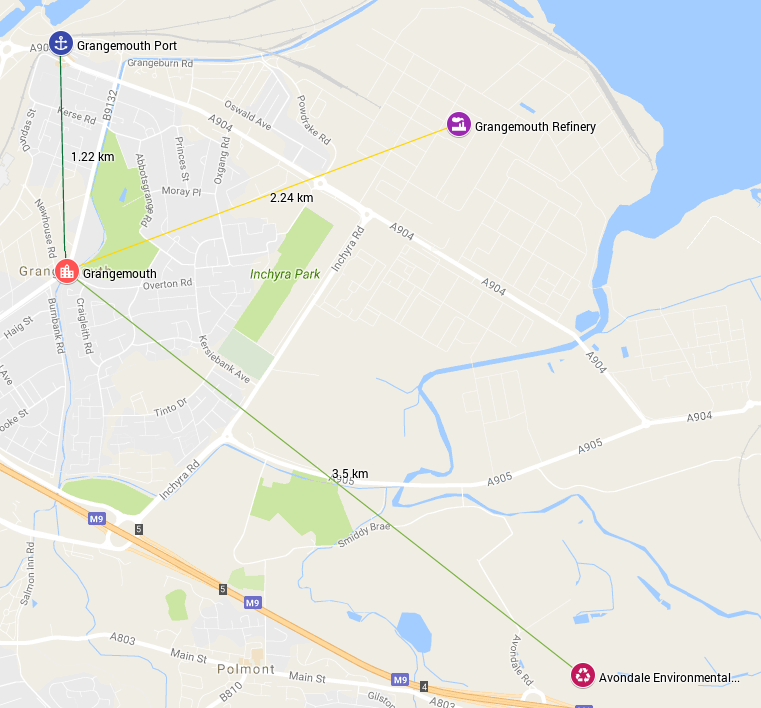
\includegraphics[width=\textwidth]{data/grangemouthmap}
    \caption{Map of Grangemouth Surroundings}
    \label{fig:grangemouthmap}
\end{figure}


\subsection{Grangemouth in Social Media}
\label{subsec:media}

Some public posts mentioning Grangemouth can be found among the public posts on such social media platforms as Facebook and Twitter, although the amount of these posts is relatively small due to the low number of people living in that area.

Some of these posts talk about environmental issues, too, however, it is important to note that there is no official communication channel established by any of the organisations which could be interested in the environmental issues in the Grangemouth area. So, in most of the posts regarding the environmental issues, people simply complain about different aspects, without expecting these complaints to solve anything or even to receive a reply from anyone who could contribute to solving the problem.

\begin{figure}[t!]
 \centering
 \begin{minipage}{10cm}
     \centering
     \subtop[]{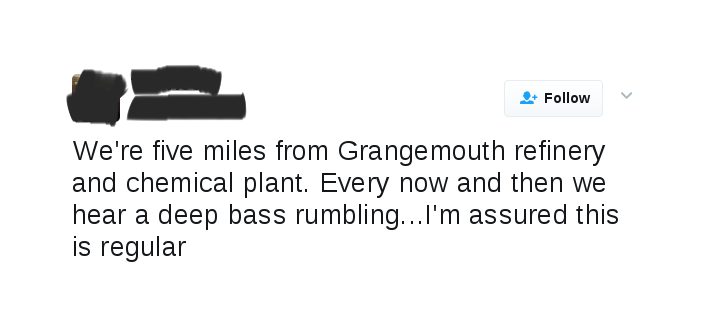
\includegraphics[width=0.8\textwidth]{data/tw1}\label{sf:tw1}}
 \end{minipage}
 \hspace{0.5cm}
 \begin{minipage}{10cm}
     \centering
     \subtop[]{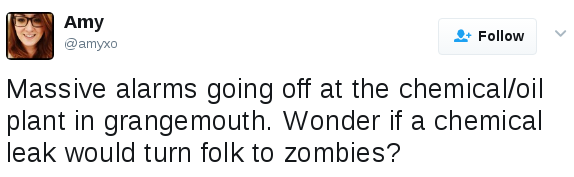
\includegraphics[width=0.8\textwidth]{data/tw2}\label{sf:tw2}}
 \end{minipage}
 \hspace{1.3cm}
 \begin{minipage}{10cm}
     \centering
     \subtop[]{
\includegraphics[width=0.8\textwidth]{data/tw3}\label{sf:tw3}}
 \end{minipage}
 \\ \vspace{0.1cm}
 \begin{minipage}{10cm}
     \centering
     \subtop[]{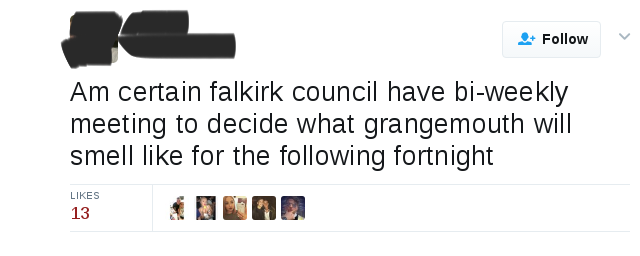
\includegraphics[width=0.8\textwidth]{data/tw4}\label{sf:tw4}}
 \end{minipage}
 \\ \vspace{0.1cm}
 \begin{minipage}{10cm}
     \centering
     \subtop[]{
\includegraphics[width=0.8\textwidth]{data/tw5}\label{sf:tw5}}
 \end{minipage}
 \mycaption[Tweet examples]{Examples of Tweets mentioning Grangemouth.}
 \label{fig:multifigtweets}
 \end{figure}
 
 Some of the examples of tweets mentioning environmental issues can be seen in figures \ref{sf:tw1} - \ref{sf:tw5}. Overall, several things could be noted when talking about such posts:
 \begin{itemize}
     \item Such posts are quite rare, one can find one or two posts every two weeks, on average
     \item Twitter is more popular among those who prefer to post about the environment publicly then Facebook
     \item Even when mentioning the environment, people use sarcasm and irony a lot, which would make it harder for a natural language processing technique to detect the correct context. In addition, people joke about the possible effects the Grangemouth refinery can have on their health.  
     \item No processing of social media data has been done by any of the companies causing the environmental disturbances or the Falkirk Council, so, supposedly, not a lot of people prefer to post about any of the problems, especially if they occur often, such as smells.
     \item People living in the Grangemouth area seem to be used to different environmental issues and are generally unhappy with them.
 \end{itemize}

\section{Project Objectives}
\label{sec:objectives}

This project is a collaboration with the Falkirk Council. The main goal of the project, as well as some of the details, have been defined by the Falkirk Council.

The main goal of the project is to create a tool that would act as an additional sensor by gathering and processing data from the social media and notifying the council in case of serious complaints about the environmental situation in the Grangemouth area. 

The objectives of the project have been outlined initially and separated into two groups: primary objectives and secondary objectives.

The \textbf{primary objectives} are the following:
\begin{itemize}
    \item Extract the existing data from Twitter. 
    \item Study the existing text classification techniques, compare them and identify those that could be used for the current project.
    \item Train a model that recognises negative tweets about Grangemouth.
\end{itemize}

The \textbf{secondary objectives} of the project build upon the primary ones and expand the performance of the model to also recognise the topic of the tweets:
\begin{itemize}
    \item Create a mechanism to send the selected tweets to the Falkirk Council as notifications. 
    \item Train another model.
    \item Analyse and compare the models and their effectiveness.
    \item Create a live tool that will receive a stream of tweets and classify them `on the go'.
    \item Look into existing studies of detecting irony and sarcasm in text.
\end{itemize}

\section{Extent of completeness}
\label{sec:completeness}

All of the primary and secondary objectives have been implemented. The rest of the report will discuss in details the techniques used in this project and how every objective was met. 
